\documentclass[main.tex]{subfiles}
\newcommand\chapterlabel{Ch-solutions}\setcounter{figurenewcounter}{0}\setcounter{tablenewcounter}{0}\setcounter{formulanewcounter}{0}\chapterpicture{../{\chapterlabel}/figure1}\chapterpicturelabel{PxFuel}


\begin{document}
  
 \setcounter{chapter}{1}\import{../\chapterlabel/files/}{ChapterName}


%      \begin{marginfigure}
%      \begin{tikzpicture} \node (a) at (0,0) {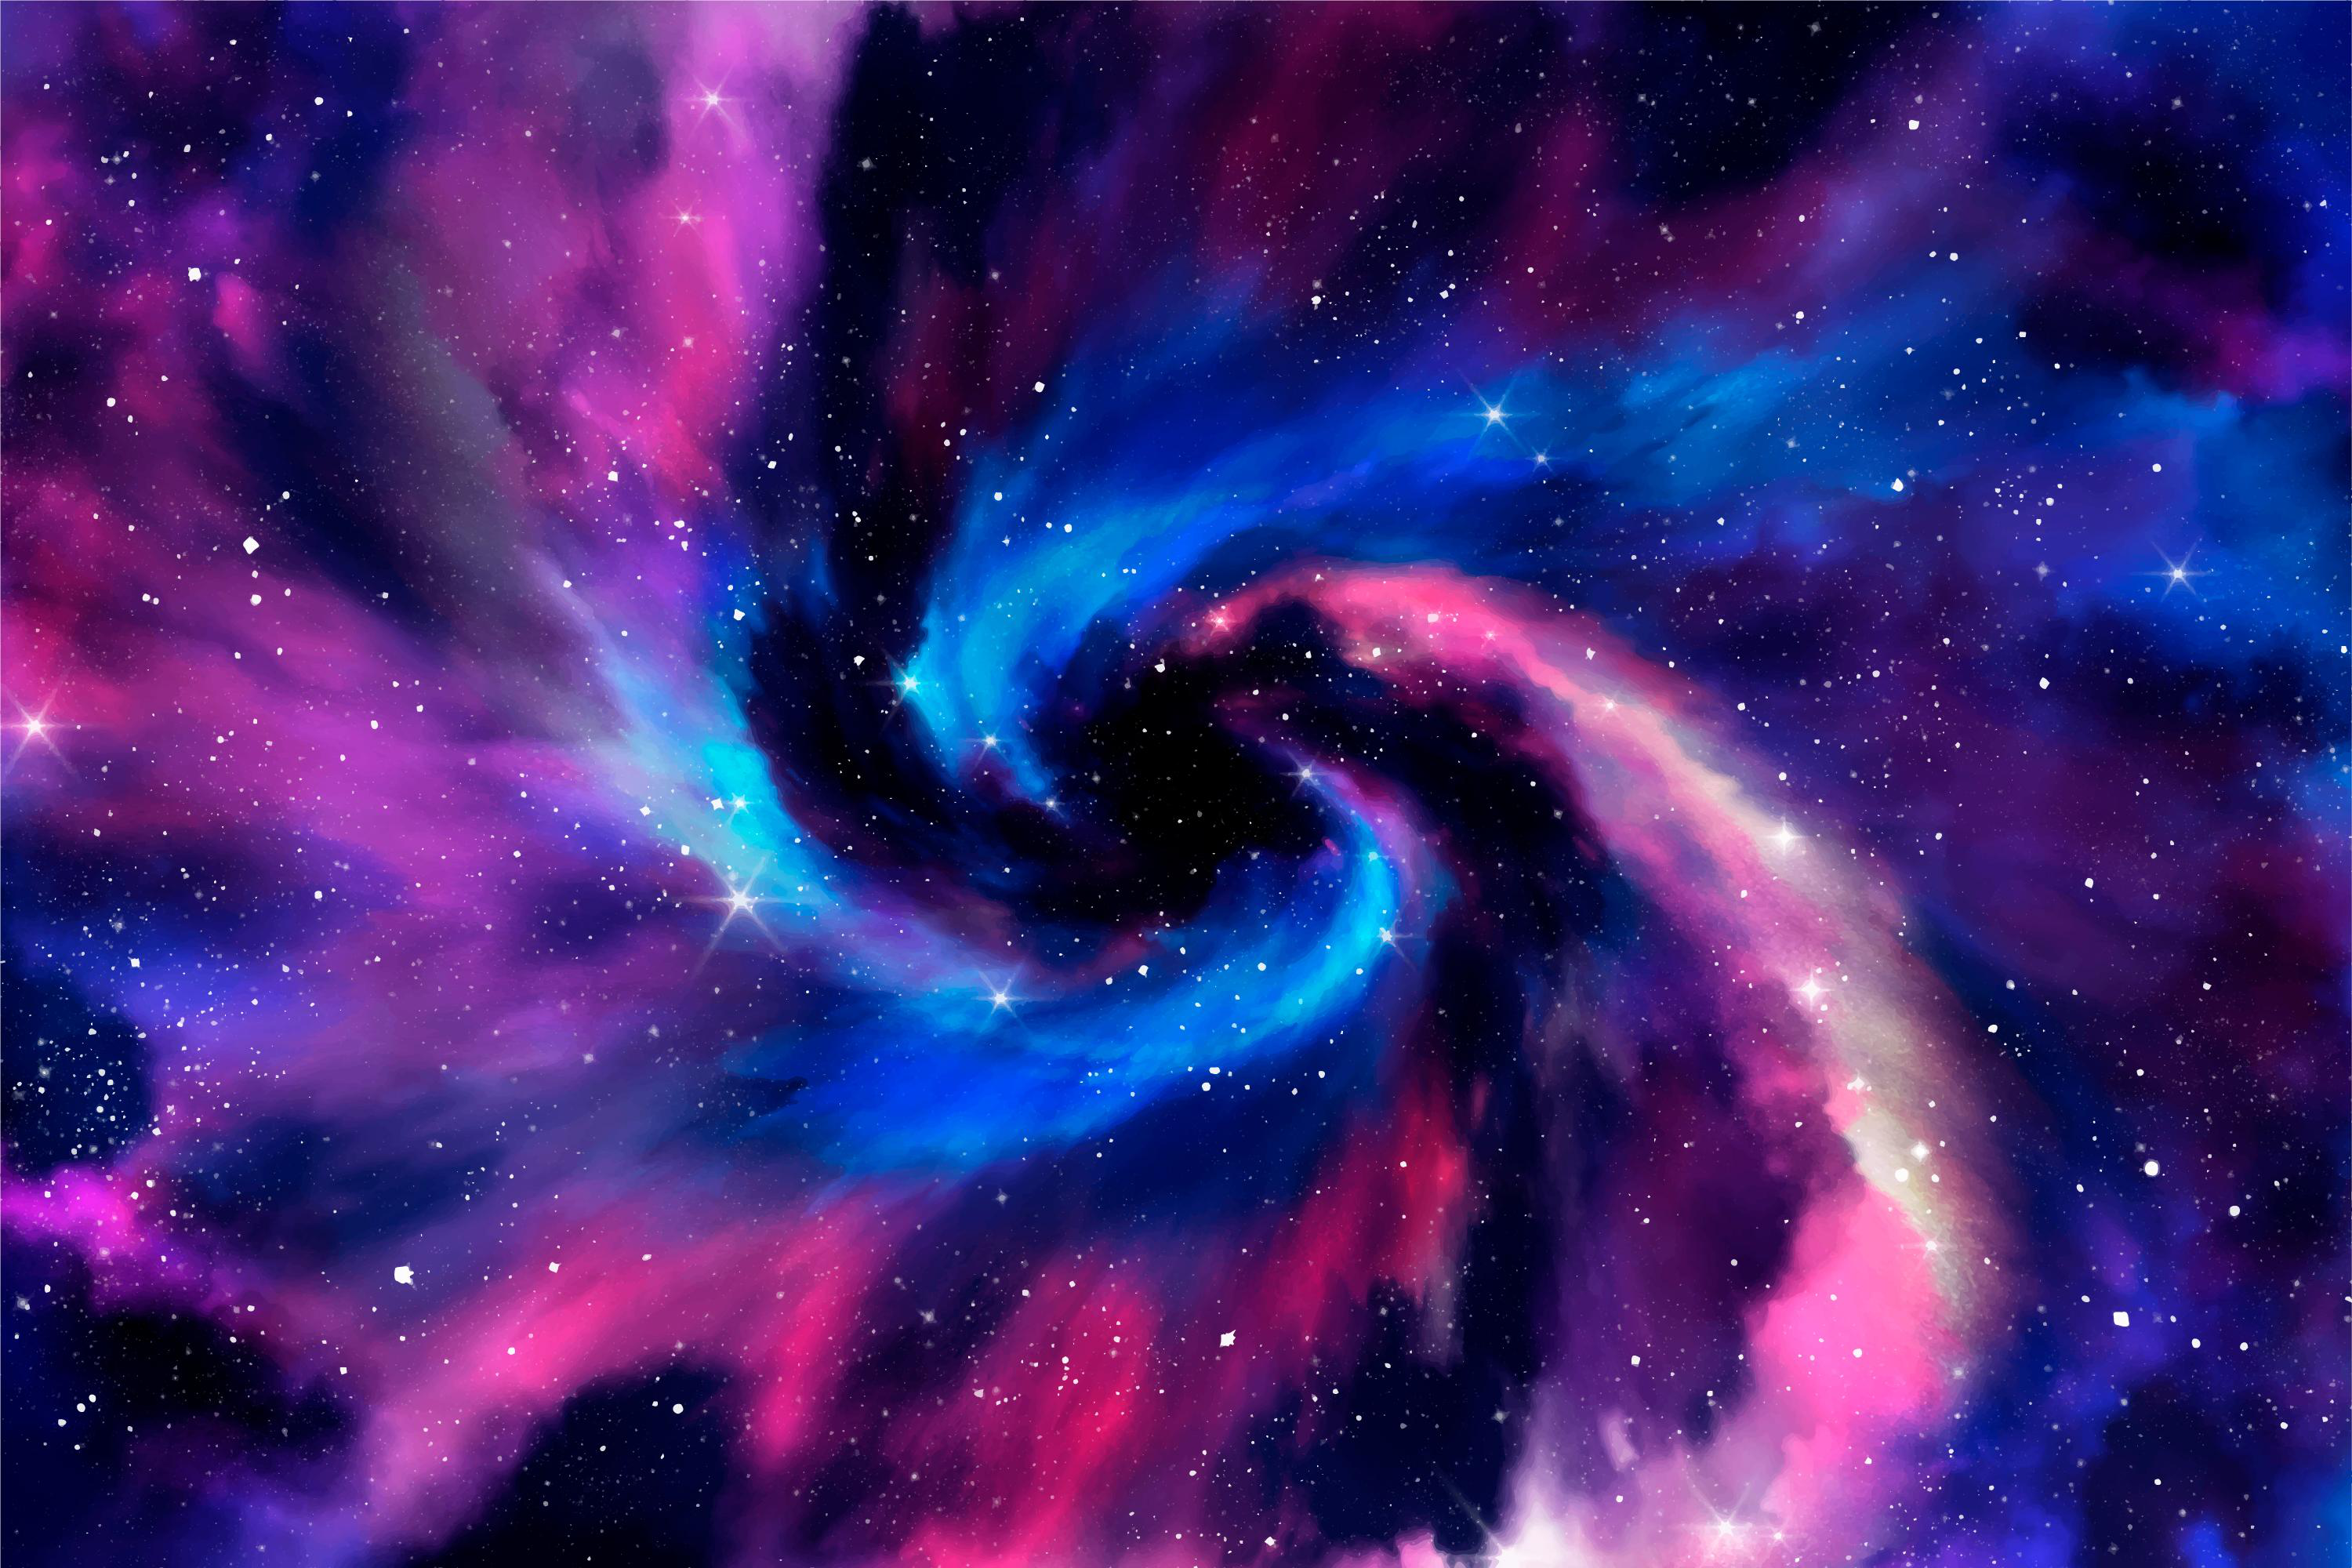
\includegraphics[width=4cm]{../Ch-solutions/figure1}} node[rotate=90, font=\tiny] at ([yshift=.5cm,xshift=.1cm]a.south east) {\textsuperscript{\textcopyright} PxFuel} ;
%\end{tikzpicture}
%\end{marginfigure}
\import{../\chapterlabel/files/}{ChapterIntro}


%\begin{marginfigure}%LEARNING GOALS BOX
%\begin{mytcbox}{GOALS}
%\begin{enumerate}[label=\protect\circled{\color{white}\arabic*}]
%\import{../\chapterlabel/files/}{SectionGoal-Colligative-properties}
%\import{../\chapterlabel/files/}{SectionGoal-Factors-affecting-the-solubility-of-solids-and-gases}
%\import{../\chapterlabel/files/}{SectionGoal-Solutions-and-colloids}
%\import{../\chapterlabel/files/}{SectionGoal-Solutions-of-electrolytes-and-effective-solute-particles}
%\import{../\chapterlabel/files/}{SectionGoal-Units-of-concentration}
%\end{enumerate}
%\end{mytcbox}
%\vspace{1cm}
%\begin{tcolorbox}[enhanced,colback=red!5!white,colframe=black!50!red,boxrule=1pt,
%  arc=0pt,outer arc=0pt,drop heavy lifted shadow]
%\faGears\ 
%\import{../\chapterlabel/files/}{ChapterDiscussion}
%
%
%
%
%
%\end{tcolorbox}
%\end{marginfigure}%LEARNING GOALS BOX



\section{Solutions and colloids}\import{../\chapterlabel/files/}{SectionIntro-Solutions-and-colloids}
\sloppy \begin{description}
\item[\docfilehook{Solutions in terms of phase and solubility}{}] \import{../\chapterlabel/files/}{Subsection-Solutions-and-colloids-Solutions-in-terms-of-phase-and-solubility}
\import{../\chapterlabel/files/}{Table-Solutions}
\item[\docfilehook{Solutions}{}] \import{../\chapterlabel/files/}{Subsection-Solutions-and-colloids-Solutions}
\item[\docfilehook{Suspensions}{}] 
\import{../\chapterlabel/files/}{Subsection-Solutions-and-colloids-Suspensions}
\import{../\chapterlabel/files/}{Figure-Colloids-diagram}
\import{../\chapterlabel/files/}{SideFigure-Colloids}
\item[\docfilehook{Colloids}{}] \import{../\chapterlabel/files/}{Subsection-Solutions-and-colloids-Colloids}
\import{../\chapterlabel/files/}{Table-Colloids}
\end{description}








\section{Units of concentration}\import{../\chapterlabel/files/}{SectionIntro-Units-of-concentration}
\sloppy \begin{description}
\item[\docfilehook{The concept of solution}{}] 
\import{../\chapterlabel/files/}{Subsection-Units-of-concentration-The-concept-of-solution}
\item[\docfilehook{Molarity, $\text{M}$}{}] \import{../\chapterlabel/files/}{Subsection-Units-of-concentration-Molarity}
\item[\docfilehook{Mole fraction, $\chi$}{}] \import{../\chapterlabel/files/}{Subsection-Units-of-concentration-Mole-fraction}
\item[\docfilehook{Percent by mass, $\%_m$}{}] \import{../\chapterlabel/files/}{Subsection-Units-of-concentration-Percent-by-mass}
\item[\docfilehook{Molality, m}{}] \import{../\chapterlabel/files/}{Subsection-Units-of-concentration-Molality}
\item[\docfilehook{Density of a solution, d}{}] \import{../\chapterlabel/files/}{Subsection-Units-of-concentration-Density}
\import{../\chapterlabel/problems/}{SampleProblem1}
\item[\docfilehook{Why relating units of concentration}{}] \import{../\chapterlabel/files/}{Subsection-Units-of-concentration-Why-relating-units-of-concentration}
\item[\docfilehook{Relating molarity and molality, $\text{M }\longleftrightarrow\text{ m}$}{}] \import{../\chapterlabel/files/}{Subsection-Units-of-concentration-Relating-M-and-m}
\item[\docfilehook{Relating molarity and the percent by mass of solute, $\text{M }\longleftrightarrow\%_{m}$}{}] \import{../\chapterlabel/files/}{Subsection-Units-of-concentration-Relating-M-and-percent}
\import{../\chapterlabel/files/}{Figure-diagram-molarity-molalilty}
\item[\docfilehook{Relating percent by mass and mole fraction of solute, $\chi \longleftrightarrow\%_{m}$}{}] 
\import{../\chapterlabel/files/}{Subsection-Units-of-concentration-Relating-percent-and-mole-fraction}
\import{../\chapterlabel/problems/}{SampleProblem2}
\item[\docfilehook{Compute molecular masses from molality and molarity}{}] 
\import{../\chapterlabel/files/}{Subsection-Units-of-concentration-Compute-molecular-masses-from-m-and-M}
\import{../\chapterlabel/problems/}{SampleProblem3}
\end{description}



\section{Solutions of electrolytes and effective solute particles}
\import{../\chapterlabel/files/}{SectionIntro-Solutions-of-electrolytes-and-effective-solute-particles}
\sloppy \begin{description}
\item[\docfilehook{Strong electrolytes}{}] \import{../\chapterlabel/files/}{Subsection-Solutions-of-electrolytes-and-effective-solute-particles-Strong-and-non-electrolytes}
\item[\docfilehook{Nonelectrolytes and weak electrolytes}{Nonelectrolytes}] \import{../\chapterlabel/files/}{Subsection-Solutions-of-electrolytes-and-effective-solute-particles-Non-electrolytes}
\item[\docfilehook{Breaking down electrolytes into ions}{}] 
\import{../\chapterlabel/files/}{Subsection-Solutions-of-electrolytes-and-effective-solute-particles-Breaking-down-electrolytes-into-ions}
\import{../\chapterlabel/problems/}{SampleProblem4}
\import{../\chapterlabel/files/}{Table-VantHoff-factors}
\item[\docfilehook{Van't Hoff factor $i$}{ }] \import{../\chapterlabel/files/}{Subsection-Solutions-of-electrolytes-and-effective-solute-particles-Vant-Hoff-factor-i}
\import{../\chapterlabel/problems/}{SampleProblem5}
\end{description}


\section{Colligative properties}\import{../\chapterlabel/files/}{SectionIntro-Colligative-properties}
\import{../\chapterlabel/files/}{Figure-Colligative-properties-phase-diagram}
\sloppy \begin{description}
\import{../\chapterlabel/files/}{SideFigure-Colligative-properties}
\item[\docfilehook{Boiling point elevation}{}] \import{../\chapterlabel/files/}{Subsection-Colligative-properties-Boiling-point-elevation}
\item[\docfilehook{Freezing point depression}{}] \import{../\chapterlabel/files/}{Subsection-Colligative-properties-Freezing-point-depression}
\import{../\chapterlabel/files/}{Table-Colligative}
\import{../\chapterlabel/problems/}{SampleProblem6}
\item[\docfilehook{Vapor-pressure lowering}{}] \import{../\chapterlabel/files/}{Subsection-Colligative-properties-Vapor-pressure-lowering}
\import{../\chapterlabel/problems/}{SampleProblem7}
\import{../\chapterlabel/files/}{Figure-Vapor-pressure-liquids}
\item[\docfilehook{Ideal and real liquid mixtures}{}] \import{../\chapterlabel/files/}{Subsection-Colligative-properties-Ideal-and-real-mixtures}
\item[\docfilehook{Osmosis}{}] \import{../\chapterlabel/files/}{Subsection-Colligative-properties-Osmosis}
\vspace{0cm}\import{../\chapterlabel/files/}{Figure-Osmosis}

\item[\docfilehook{Isotonic, hypotonic and hypertonic solutions}{}] \import{../\chapterlabel/files/}{Subsection-Colligative-properties-Isotonic-hypotonic-and-hypertonic-solutions}
\item[\docfilehook{Dialisis}{}] \import{../\chapterlabel/files/}{Subsection-Colligative-properties-Dialisis}

\item[\docfilehook{Osmotic pressure of a solution}{}] \import{../\chapterlabel/files/}{Subsection-Colligative-properties-Osmotic-pressure}
\import{../\chapterlabel/files/}{SideFigure-dialisis}
\item[\docfilehook{Osmolarity}{}] \import{../\chapterlabel/files/}{Subsection-Colligative-properties-Osmolarity}
\item[\docfilehook{Colligative properties review}{}] \import{../\chapterlabel/files/}{Subsection-Colligative-properties-Colligative-properties-review}
\item[\docfilehook{Graphical method to calculate colligative constants}{}] \import{../\chapterlabel/files/}{Subsection-Colligative-properties-Graphical-method-to-calculate-colligative-constants}
\import{../\chapterlabel/problems/}{SampleProblem8}
\item[\docfilehook{Use of colligative properties to calculate $\alpha$}{}] \import{../\chapterlabel/files/}{Subsection-Colligative-properties-Use-of-Colligative-properties-to-calclate-alpha}
\import{../\chapterlabel/problems/}{SampleProblem9}
\item[\docfilehook{Use of colligative properties to calculate $MW$}{}] \import{../\chapterlabel/files/}{Subsection-Colligative-properties-Use-of-Colligative-properties-to-calculate-MW}
\import{../\chapterlabel/problems/}{SampleProblem10}
\end{description}




\section{Factors affecting the solubility of solids and gases}\import{../\chapterlabel/files/}{SectionIntro-Factors-affecting-the-solubility-of-solids-and-gases}
\sloppy \begin{description}
\item[\docfilehook{Impact of the molecular structure on solubility }{}] \import{../\chapterlabel/files/}{Subsection-Factors-affecting-the-solubility-of-solids-and-gases-Impact-of-the-molecular-structure-on-solubility}
\item[\docfilehook{Impact of temperature on solubility }{}] \import{../\chapterlabel/files/}{Subsection-Factors-affecting-the-solubility-of-solids-and-gases-Impact-of-the-temperature-on-solubility}
\item[\docfilehook{Impact of pressure on the solubility of gases on liquids}{}] \import{../\chapterlabel/files/}{Subsection-Factors-affecting-the-solubility-of-solids-and-gases-Impact-of-the-pressure-on-solubility-of-gases-on-liquids}
\import{../\chapterlabel/problems/}{SampleProblem11}
\end{description}


\checkoddpage\ifoddpage \clearpage\thispagestyle{empty}\mbox{}\clearpage \else  \fi \end{document}

